% Principal GDZ PPN236018647, native 458–459; HKUST 459–460.
\SourceLeaf{458}\NoSourceHead
\pdfbookmark[1]{Ansätze zur transzendenten Trigonometrie}{transzendente-trigonometrie}
\HistoricTitle{NACHLASS.}
\bigskip
\HistoricTitle{[ANSÄTZE ZUR TRANSZENDENTEN TRIGONOMETRIE.]}
\HistoricCitation{[Aus Scheda Af, Mémoires de Mathématique, Bronsuic 1801.]}
\SourceGroup{I}
\noindent [S. 68]\par\smallskip
\noindent\begin{minipage}[c]{.68\linewidth}
\[
\begin{aligned}
\omega\partial\psi\Delta&=2i\psi(\omega\varphi\Delta)\\
\partial\Delta&=i\varphi(\omega\varphi\Delta)\\
\varphi(\omega\varphi\Delta)\omega\partial\psi\Delta&=2\partial\Delta\mathbin{.}\psi(\omega\varphi\Delta)\\
\psi'\Delta&=\frac{2\psi(\omega\varphi\Delta)}{\omega\varphi(\omega\varphi\Delta)}\\
\chi'\Delta&=\varphi\Delta\\
\psi'\Delta&=\frac{2\psi\{\omega\chi'\Delta\}}{\omega\chi'\{\omega\chi'\Delta\}}\\
\psi'\Delta\mathbin{.}\alpha\omega\omega\chi'\Delta&=2\beta\omega\omega\chi'\Delta^2\\
\alpha\psi'\Delta&=2[\beta]\chi'\Delta.
\end{aligned}
\]
\end{minipage}\hfill\begin{minipage}[c]{.30\linewidth}\centering
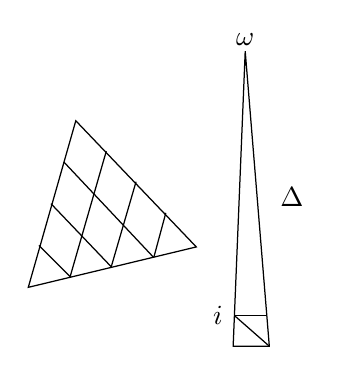
\begin{tikzpicture}[x=.009cm,y=-.009cm,line width=.45pt]
\draw (33,383)--(100,148)--(270,326)--cycle;
\draw (83,206)--(210,341);
\draw (65,265)--(150,354);
\draw (48,324)--(92,368);
\draw (143,191)--(92,368);
\draw (185,234)--(150,354);
\draw (227,278)--(210,341);
\draw (339,50)--(322,466)--(373,466)--cycle;
\draw (324,423)--(370,423);
\draw (324,423)--(373,466);
\node[above,inner sep=2pt] at (339,50) {$\omega$};
\node[right,inner sep=2pt] at (380,255) {$\Delta$};
\node[left,inner sep=2pt] at (316,423) {$i$};
\end{tikzpicture}
\end{minipage}
\SourceGroup{II}
\begin{center}
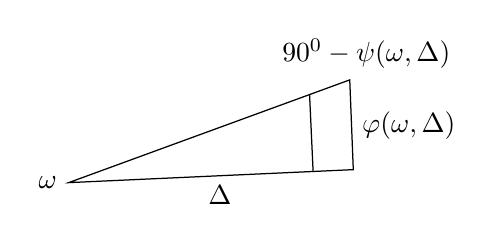
\begin{tikzpicture}[x=.015cm,y=-.015cm,line width=.45pt]
\draw (0,99)--(238,12)--(241,88)--cycle;
\draw (204,25)--(207,90);
\node[left,inner sep=4pt] at (0,99) {$\omega$};
\node[below,inner sep=3pt] at (128,94) {$\Delta$};
\node[right,inner sep=3pt] at (241,51) {$\varphi(\omega,\Delta)$};
\node[above,inner sep=4pt] at (252,12) {$90^{0}-\psi(\omega,\Delta)$};
\end{tikzpicture}
\end{center}
\[
\frac{\partial\varphi(\omega,\Delta)}{\partial\Delta}=\psi(\omega,\Delta).
\]
\par\medskip\noindent\hfill 57\textsuperscript{*}
\clearpage\SourceLeaf{459}\ArithmeticHead{452}{L}{GEOMETRIE. NACHLASS.}
\noindent [S. 69]
\SourceGroup{III}
\begin{center}
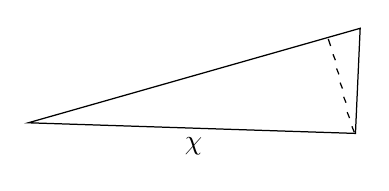
\begin{tikzpicture}[x=.015cm,y=-.015cm,line width=.45pt]
\draw (0,99)--(281,19)--(277,108)--cycle;
\draw (254,28)--(256,34);
\draw (258,41)--(260,46);
\draw (261,53)--(263,58);
\draw (264,65)--(266,70);
\draw (267,77)--(269,82);
\draw (270,90)--(272,95);
\draw (274,102)--(276,107);
\node[below,inner sep=3pt] at (140,104) {$\chi$};
\end{tikzpicture}
\end{center}
\[
\begin{gathered}
\varphi(\omega,\Delta)\\
\psi\{\omega,\chi(\omega,\Delta)\}
\end{gathered}
\]
\[
\begin{aligned}
\Delta&=\chi\{\omega,\chi(\omega,\Delta)\}+\varphi\{\psi(\omega,\chi(\omega,\Delta)),\varphi(\omega,\Delta)\}\\
\psi(\omega,\Delta)&=\psi\{\psi(\omega,\chi(\omega,\Delta)),\varphi(\omega,\Delta)\}\\
\varphi\{\omega,\chi(\omega,\Delta)\}&=\chi\{\psi(\omega,\chi(\omega,\Delta)),\varphi(\omega,\Delta)\}\\
\varphi(\omega,\Delta)&=\omega f\Delta+\omega\omega f'\Delta\\
\chi(\omega,\Delta)&=\Delta+\omega g\Delta+\omega\omega g'\Delta\\
\psi(\omega,\Delta)&=\omega+\omega\omega h'\Delta.
\end{aligned}
\]
\clearpage
\noindent [S. 70]
\SourceGroup{IV}
\begin{center}
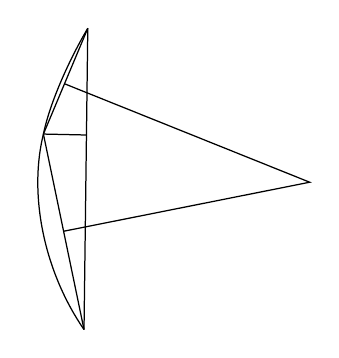
\begin{tikzpicture}[x=.012cm,y=-.012cm,line width=.45pt]
\draw (67,8)--(63,327);
\draw (67,8)--(20,120)--(63,327);
\draw (67,8)..controls (48,40) and (27,86)..(20,120)..controls (4,185) and (21,266)..(63,327);
\draw (20,120)--(66,121);
\draw (43,67)--(302,171)--(41,223);
\end{tikzpicture}
\end{center}
\[
\begin{aligned}
&\varphi\{2\varphi(\Delta,\tfrac12 a),\ \psi(\Delta,\tfrac12(a+b))-\psi(\Delta,\tfrac12 a)\}\\
&\quad=\varphi\{2\varphi(\Delta,\tfrac12 b),\ \psi(\Delta,\tfrac12(a+b))-\psi(\Delta,\tfrac12 b)\}
\end{aligned}
\]
\[
\begin{aligned}
&\psi\{2\varphi(\Delta,\tfrac12 a),\ \psi(\Delta,\tfrac12(a+b))-\psi(\Delta,\tfrac12 a)\}\\
&\quad+\psi\{2\varphi(\Delta,\tfrac12 b),\ \psi(\Delta,\tfrac12(a+b))-\psi(\Delta,\tfrac12 b)\}\\
&\qquad=\psi(\Delta,\tfrac12 a)+\psi(\Delta,\tfrac12 b)
\end{aligned}
\]
\[
\begin{aligned}
&\varphi\{2\varphi(\Delta,\tfrac12 a),\ \psi^{0,1}(\Delta,\tfrac12 a)\partial\tfrac12 a\}\\
&\quad=\varphi\{2\varphi(\Delta,\tfrac12\partial a),\ \psi(\Delta,\tfrac12 a)\}
\end{aligned}
\]
\[
\begin{aligned}
\varphi(\Delta,a)&=\Delta f a+\Delta^3 f'a\\
\psi(\Delta,a)&=a+\Delta\Delta g a.
\end{aligned}
\]
